% Options for packages loaded elsewhere
\PassOptionsToPackage{unicode}{hyperref}
\PassOptionsToPackage{hyphens}{url}
\documentclass[
  ignorenonframetext,
]{beamer}
\newif\ifbibliography
\usepackage{pgfpages}
\setbeamertemplate{caption}[numbered]
\setbeamertemplate{caption label separator}{: }
\setbeamercolor{caption name}{fg=normal text.fg}
\beamertemplatenavigationsymbolsempty
% remove section numbering
\setbeamertemplate{part page}{
  \centering
  \begin{beamercolorbox}[sep=16pt,center]{part title}
    \usebeamerfont{part title}\insertpart\par
  \end{beamercolorbox}
}
\setbeamertemplate{section page}{
  \centering
  \begin{beamercolorbox}[sep=12pt,center]{section title}
    \usebeamerfont{section title}\insertsection\par
  \end{beamercolorbox}
}
\setbeamertemplate{subsection page}{
  \centering
  \begin{beamercolorbox}[sep=8pt,center]{subsection title}
    \usebeamerfont{subsection title}\insertsubsection\par
  \end{beamercolorbox}
}
% Prevent slide breaks in the middle of a paragraph
\widowpenalties 1 10000
\raggedbottom
\AtBeginPart{
  \frame{\partpage}
}
\AtBeginSection{
  \ifbibliography
  \else
    \frame{\sectionpage}
  \fi
}
\AtBeginSubsection{
  \frame{\subsectionpage}
}
\usepackage{iftex}
\ifPDFTeX
  \usepackage[T1]{fontenc}
  \usepackage[utf8]{inputenc}
  \usepackage{textcomp} % provide euro and other symbols
\else % if luatex or xetex
  \usepackage{unicode-math} % this also loads fontspec
  \defaultfontfeatures{Scale=MatchLowercase}
  \defaultfontfeatures[\rmfamily]{Ligatures=TeX,Scale=1}
\fi
\usepackage{lmodern}
\ifPDFTeX\else
  % xetex/luatex font selection
\fi
% Use upquote if available, for straight quotes in verbatim environments
\IfFileExists{upquote.sty}{\usepackage{upquote}}{}
\IfFileExists{microtype.sty}{% use microtype if available
  \usepackage[]{microtype}
  \UseMicrotypeSet[protrusion]{basicmath} % disable protrusion for tt fonts
}{}
\makeatletter
\@ifundefined{KOMAClassName}{% if non-KOMA class
  \IfFileExists{parskip.sty}{%
    \usepackage{parskip}
  }{% else
    \setlength{\parindent}{0pt}
    \setlength{\parskip}{6pt plus 2pt minus 1pt}}
}{% if KOMA class
  \KOMAoptions{parskip=half}}
\makeatother
\usepackage{color}
\usepackage{fancyvrb}
\newcommand{\VerbBar}{|}
\newcommand{\VERB}{\Verb[commandchars=\\\{\}]}
\DefineVerbatimEnvironment{Highlighting}{Verbatim}{commandchars=\\\{\}}
% Add ',fontsize=\small' for more characters per line
\newenvironment{Shaded}{}{}
\newcommand{\AlertTok}[1]{\textcolor[rgb]{1.00,0.00,0.00}{\textbf{#1}}}
\newcommand{\AnnotationTok}[1]{\textcolor[rgb]{0.38,0.63,0.69}{\textbf{\textit{#1}}}}
\newcommand{\AttributeTok}[1]{\textcolor[rgb]{0.49,0.56,0.16}{#1}}
\newcommand{\BaseNTok}[1]{\textcolor[rgb]{0.25,0.63,0.44}{#1}}
\newcommand{\BuiltInTok}[1]{\textcolor[rgb]{0.00,0.50,0.00}{#1}}
\newcommand{\CharTok}[1]{\textcolor[rgb]{0.25,0.44,0.63}{#1}}
\newcommand{\CommentTok}[1]{\textcolor[rgb]{0.38,0.63,0.69}{\textit{#1}}}
\newcommand{\CommentVarTok}[1]{\textcolor[rgb]{0.38,0.63,0.69}{\textbf{\textit{#1}}}}
\newcommand{\ConstantTok}[1]{\textcolor[rgb]{0.53,0.00,0.00}{#1}}
\newcommand{\ControlFlowTok}[1]{\textcolor[rgb]{0.00,0.44,0.13}{\textbf{#1}}}
\newcommand{\DataTypeTok}[1]{\textcolor[rgb]{0.56,0.13,0.00}{#1}}
\newcommand{\DecValTok}[1]{\textcolor[rgb]{0.25,0.63,0.44}{#1}}
\newcommand{\DocumentationTok}[1]{\textcolor[rgb]{0.73,0.13,0.13}{\textit{#1}}}
\newcommand{\ErrorTok}[1]{\textcolor[rgb]{1.00,0.00,0.00}{\textbf{#1}}}
\newcommand{\ExtensionTok}[1]{#1}
\newcommand{\FloatTok}[1]{\textcolor[rgb]{0.25,0.63,0.44}{#1}}
\newcommand{\FunctionTok}[1]{\textcolor[rgb]{0.02,0.16,0.49}{#1}}
\newcommand{\ImportTok}[1]{\textcolor[rgb]{0.00,0.50,0.00}{\textbf{#1}}}
\newcommand{\InformationTok}[1]{\textcolor[rgb]{0.38,0.63,0.69}{\textbf{\textit{#1}}}}
\newcommand{\KeywordTok}[1]{\textcolor[rgb]{0.00,0.44,0.13}{\textbf{#1}}}
\newcommand{\NormalTok}[1]{#1}
\newcommand{\OperatorTok}[1]{\textcolor[rgb]{0.40,0.40,0.40}{#1}}
\newcommand{\OtherTok}[1]{\textcolor[rgb]{0.00,0.44,0.13}{#1}}
\newcommand{\PreprocessorTok}[1]{\textcolor[rgb]{0.74,0.48,0.00}{#1}}
\newcommand{\RegionMarkerTok}[1]{#1}
\newcommand{\SpecialCharTok}[1]{\textcolor[rgb]{0.25,0.44,0.63}{#1}}
\newcommand{\SpecialStringTok}[1]{\textcolor[rgb]{0.73,0.40,0.53}{#1}}
\newcommand{\StringTok}[1]{\textcolor[rgb]{0.25,0.44,0.63}{#1}}
\newcommand{\VariableTok}[1]{\textcolor[rgb]{0.10,0.09,0.49}{#1}}
\newcommand{\VerbatimStringTok}[1]{\textcolor[rgb]{0.25,0.44,0.63}{#1}}
\newcommand{\WarningTok}[1]{\textcolor[rgb]{0.38,0.63,0.69}{\textbf{\textit{#1}}}}
\usepackage{longtable,booktabs,array}
\newcounter{none} % for unnumbered tables
\usepackage{calc} % for calculating minipage widths
\usepackage{caption}
% Make caption package work with longtable
\makeatletter
\def\fnum@table{\tablename~\thetable}
\makeatother
\usepackage{graphicx}
\makeatletter
\newsavebox\pandoc@box
\newcommand*\pandocbounded[1]{% scales image to fit in text height/width
  \sbox\pandoc@box{#1}%
  \Gscale@div\@tempa{\textheight}{\dimexpr\ht\pandoc@box+\dp\pandoc@box\relax}%
  \Gscale@div\@tempb{\linewidth}{\wd\pandoc@box}%
  \ifdim\@tempb\p@<\@tempa\p@\let\@tempa\@tempb\fi% select the smaller of both
  \ifdim\@tempa\p@<\p@\scalebox{\@tempa}{\usebox\pandoc@box}%
  \else\usebox{\pandoc@box}%
  \fi%
}
% Set default figure placement to htbp
\def\fps@figure{htbp}
\makeatother
\setlength{\emergencystretch}{3em} % prevent overfull lines
\providecommand{\tightlist}{%
  \setlength{\itemsep}{0pt}\setlength{\parskip}{0pt}}
\usepackage{bookmark}
\IfFileExists{xurl.sty}{\usepackage{xurl}}{} % add URL line breaks if available
\urlstyle{same}
\hypersetup{
  pdftitle={Enriched Category Theory of Language},
  hidelinks,
  pdfcreator={LaTeX via pandoc}}

\title{\texorpdfstring{Enriched Category Theory of
Language}{Enriched Category Theory of Language}}
\author{\texorpdfstring{}{}}
\date{}

\begin{document}
\frame{\titlepage}

\section{Enriched Category Theory and Distributional Measures of
Language}\label{sec:enriched-categories}

\begin{frame}{Beyond Discrete Categories: Quantitative Grading}
\protect\phantomsection\label{beyond-discrete-categories-quantitative-grading}
The categories introduced in \autoref{sec:case-systems}---with case
roles as objects and grammatical relations as morphisms---capture the
\emph{qualitative} structure of case systems: which roles exist and how
they connect. But linguistic data is fundamentally \emph{quantitative}:
some grammatical relations are more probable than others, some role
assignments are stronger than others, and distributional similarity is a
matter of degree.

To accommodate this quantitative dimension, we move from ordinary
categories to \textbf{enriched categories}, where hom-sets are not just
sets of morphisms but carry additional algebraic structure. The
framework of Fritz et al. {[}-@fritz2021enriched{]} provides the key
construction.
\end{frame}

\begin{frame}[fragile]{The \([0,1]\)-Enrichment of Case Categories}
\protect\phantomsection\label{the-01-enrichment-of-case-categories}
\begin{block}{Definition}
\protect\phantomsection\label{definition}
A category \(\mathcal{C}\) enriched over the unit interval
\(([0,1], \cdot, 1)\) assigns to every pair of objects \(A, B\) a
\emph{hom-value} \(\mathcal{C}(A, B) \in [0,1]\) satisfying:

\begin{enumerate}
\tightlist
\item
  \textbf{Identity}: \(\mathcal{C}(A, A) = 1\) for all objects \(A\)
\item
  \textbf{Composition}:
  \(\mathcal{C}(A, C) \geq \mathcal{C}(A, B) \cdot \mathcal{C}(B, C)\)
  for all objects \(A, B, C\)
\end{enumerate}

The identity axiom says that every expression is maximally related to
itself. The composition inequality says that distributional relatedness
composes sub-multiplicatively: if \(A\) is 80\% related to \(B\) and
\(B\) is 70\% related to \(C\), then \(A\) must be at least
\(0.8 \times 0.7 = 56\%\) related to \(C\).
\end{block}

\begin{block}{Interpreting Hom-Values in Linguistic Context}
\protect\phantomsection\label{interpreting-hom-values-in-linguistic-context}
Fritz et al. {[}-@fritz2021enriched{]} interpret hom-values as
\emph{conditional probabilities} in a distributional model:
\(\mathcal{C}(A, B) = P(\text{context} \mid A \text{ and } B \text{ co-occur})\).
In our case-theoretic application, we interpret them more broadly:

{\def\LTcaptype{none} % do not increment counter
\begin{longtable}[]{@{}
  >{\raggedright\arraybackslash}p{(\linewidth - 4\tabcolsep) * \real{0.3333}}
  >{\raggedright\arraybackslash}p{(\linewidth - 4\tabcolsep) * \real{0.3333}}
  >{\raggedright\arraybackslash}p{(\linewidth - 4\tabcolsep) * \real{0.3333}}@{}}
\toprule\noalign{}
\begin{minipage}[b]{\linewidth}\raggedright
Hom-value interpretation
\end{minipage} & \begin{minipage}[b]{\linewidth}\raggedright
Domain
\end{minipage} & \begin{minipage}[b]{\linewidth}\raggedright
Example
\end{minipage} \\
\midrule\noalign{}
\endhead
Conditional probability & Corpus statistics & P(ACC role \textbar{}
transitive verb context) \\
Proto-role strength & Semantic typology & Degree of Proto-Agent
satisfaction \\
Distributional similarity & Vector semantics & Cosine similarity of
case-role embeddings \\
Morphological predictability & Morpholexicology & Reliability of
case-marking paradigm \\
\bottomrule\noalign{}
\end{longtable}
}
\end{block}

\begin{block}{Implementation via the EnrichedCategory Class}
\protect\phantomsection\label{implementation-via-the-enrichedcategory-class}
Our \texttt{EnrichedCategory} class implements this structure directly:

\begin{Shaded}
\begin{Highlighting}[]
\NormalTok{cat }\OperatorTok{=}\NormalTok{ EnrichedCategory(name}\OperatorTok{=}\StringTok{"English Case Proximity"}\NormalTok{)}
\NormalTok{cat.add\_object(}\StringTok{"NOM"}\NormalTok{)}
\NormalTok{cat.add\_object(}\StringTok{"ACC"}\NormalTok{)}
\NormalTok{cat.add\_object(}\StringTok{"DAT"}\NormalTok{)}

\NormalTok{cat.set\_hom(}\StringTok{"NOM"}\NormalTok{, }\StringTok{"ACC"}\NormalTok{, }\FloatTok{0.85}\NormalTok{)  }\CommentTok{\# high: agent/patient often co{-}occur}
\NormalTok{cat.set\_hom(}\StringTok{"ACC"}\NormalTok{, }\StringTok{"DAT"}\NormalTok{, }\FloatTok{0.45}\NormalTok{)  }\CommentTok{\# moderate: object/recipient sometimes overlap}
\NormalTok{cat.set\_hom(}\StringTok{"NOM"}\NormalTok{, }\StringTok{"DAT"}\NormalTok{, }\FloatTok{0.30}\NormalTok{)  }\CommentTok{\# low: subject/recipient rarely merge}

\CommentTok{\# Verify composition inequality: 0.30 \textgreater{}= 0.85 * 0.45 = 0.3825?}
\CommentTok{\# This fails! English NOM{-}DAT is too distant relative to the chain.}
\ControlFlowTok{assert} \KeywordTok{not}\NormalTok{ cat.check\_composition\_inequality(}\StringTok{"NOM"}\NormalTok{, }\StringTok{"ACC"}\NormalTok{, }\StringTok{"DAT"}\NormalTok{)}
\end{Highlighting}
\end{Shaded}

The composition inequality violation here is linguistically meaningful:
it tells us that the NOM→ACC→DAT chain overestimates the direct NOM→DAT
relatedness, reflecting the typological fact that subject--recipient
identity (e.g., in benefactive constructions) is more restricted than
the product of agent--patient and patient--recipient proximities.
\autoref{fig:enriched-heatmap} shows the distributional relations
between case roles as a categorical relation graph.

\begin{figure}
\centering
\pandocbounded{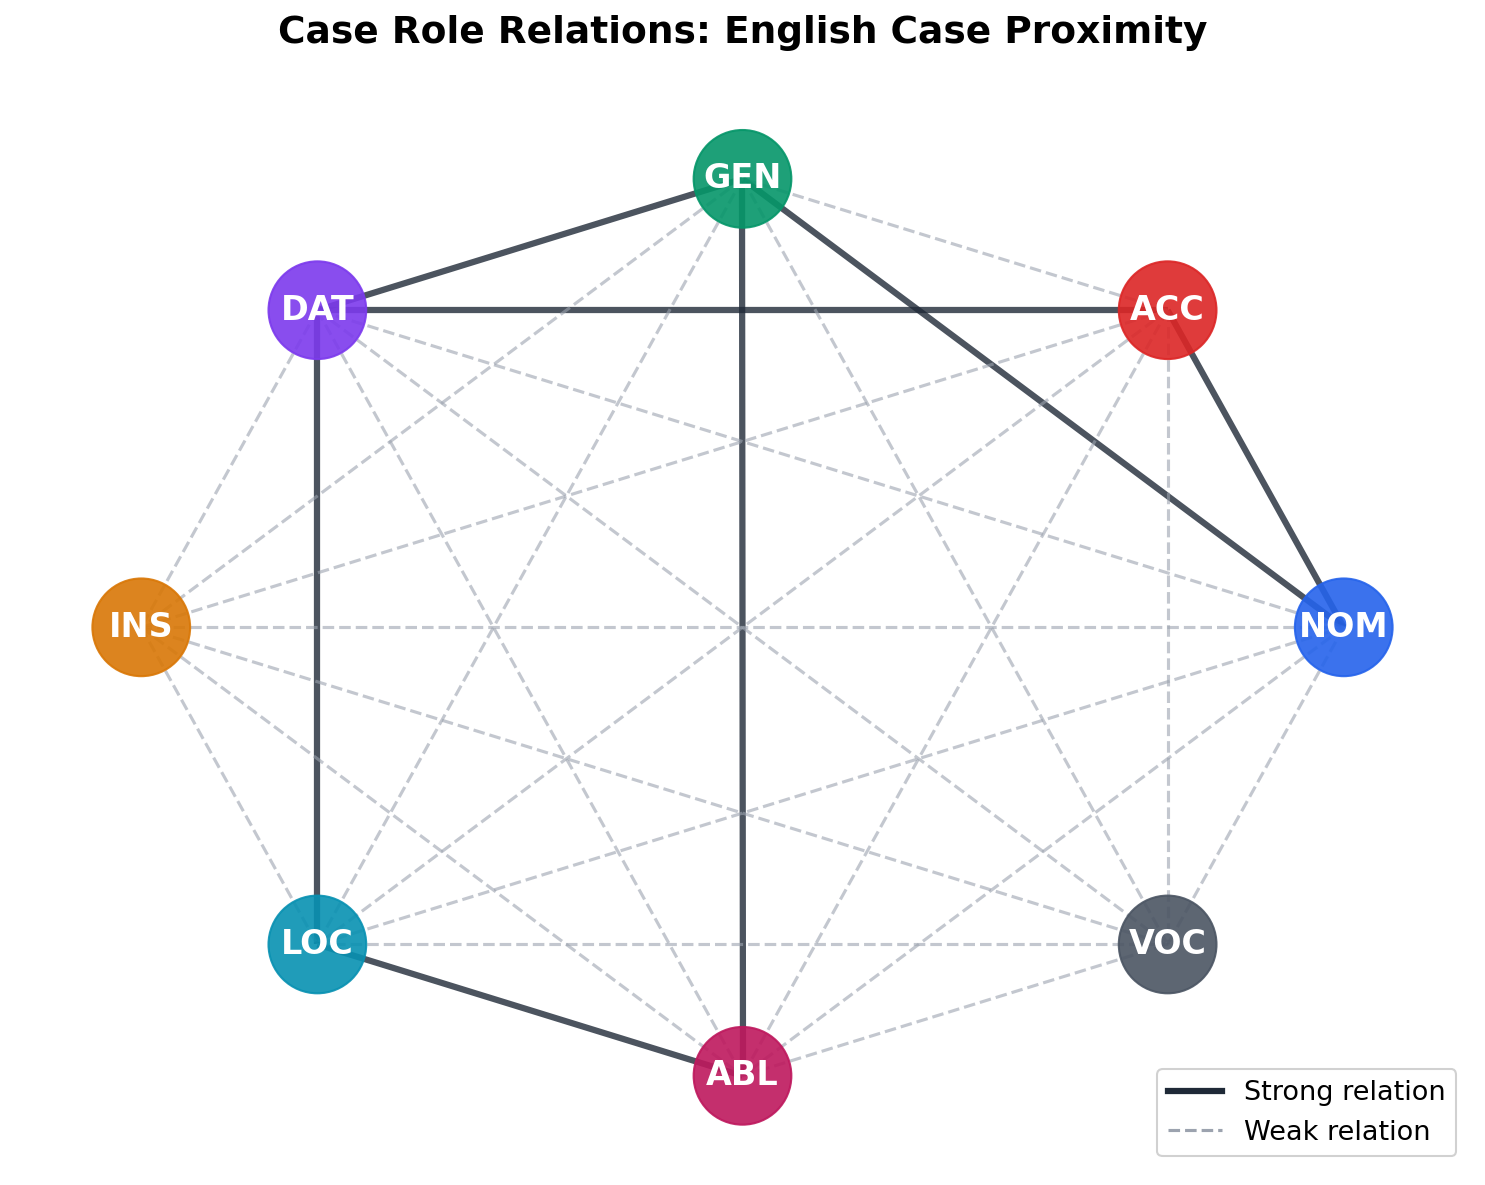
\includegraphics[keepaspectratio,alt={Case role distributional relation graph showing the network of pairwise relationships among all eight case roles (NOM, ACC, GEN, DAT, INS, LOC, ABL, VOC). Strong relations appear as solid edges (indicating frequent co-occurrence or high proto-role overlap), while weaker relations appear as dashed edges. The graph layout reveals clusters of semantically proximate roles (e.g., NOM - ACC, DAT - GEN) and the relative isolation of peripheral cases (VOC, ABL).}]{../figures/enriched_hom_matrix.png}}
\caption{Case role distributional relation graph showing the network of
pairwise relationships among all eight case roles (NOM, ACC, GEN, DAT,
INS, LOC, ABL, VOC). Strong relations appear as solid edges (indicating
frequent co-occurrence or high proto-role overlap), while weaker
relations appear as dashed edges. The graph layout reveals clusters of
semantically proximate roles (e.g., NOM - ACC, DAT - GEN) and the
relative isolation of peripheral cases (VOC,
ABL).}\label{fig:enriched-heatmap}
\end{figure}
\end{block}
\end{frame}

\begin{frame}{Categorical Magnitude as a Complexity Invariant}
\protect\phantomsection\label{categorical-magnitude-as-a-complexity-invariant}
A key invariant of enriched categories is their \textbf{magnitude}---a
numerical quantity that captures the ``effective size'' of the category,
discounting for overlap between objects.

For an enriched category with \(n\) objects, let \(Z\) be the
\(n \times n\) matrix with \(Z_{ij} = \mathcal{C}(i, j)\). The magnitude
is:

\[|\mathcal{C}| = \sum_{i,j} (Z^{-1})_{ij}\]

when \(Z\) is invertible. Magnitude has deep connections to information
theory:

\begin{itemize}
\tightlist
\item
  For a \emph{discrete} category (no non-trivial relationships),
  \(|\mathcal{C}| = n\) (the number of objects)
\item
  For a highly connected category, \(|\mathcal{C}| < n\) (objects are
  ``redundant'')
\item
  Magnitude connects to the diversity measures studied in ecology
  (species diversity), graph theory (effective graph resistance), and
  information geometry (Fisher information)
\end{itemize}

Bradley {[}-@bradley2020entropy{]} establishes a foundational link
between categorical magnitude and information entropy through
topological operad derivations. Her result shows that Shannon entropy
can be characterized as the unique derivation of a certain topological
operad---a categorical structure that also governs the composition of
enriched categories. This provides a deep theoretical justification for
using magnitude as a measure of linguistic complexity: the magnitude of
a case category quantifies how much ``information'' the case system
encodes about relational structure.
\end{frame}

\begin{frame}{Enriched Functors and Bradley's Language-as-Category
Model}
\protect\phantomsection\label{enriched-functors-and-bradleys-language-as-category-model}
Bradley's {[}-@bradley2024ipam; -@bradley2025tea{]} broader program
treats natural language itself as an enriched category, where:

\begin{itemize}
\tightlist
\item
  \textbf{Objects} are expressions (words, phrases, sentences)
\item
  \textbf{Hom-values} encode distributional co-occurrence probabilities
\item
  \textbf{Composition} models transitivity of distributional relatedness
\end{itemize}

This ``language as enriched category'' perspective has profound
implications for case theory:

\begin{enumerate}
\item
  \textbf{Case roles emerge from distributional structure}: Rather than
  being imposed a priori, case distinctions arise from clusters of high
  hom-values in the enriched language category. Nouns that frequently
  appear in agent contexts cluster together, forming the ``nominative''
  region of the category.
\item
  \textbf{Alignment types correspond to enriched structure}: Different
  languages partition the enriched category differently, and these
  partitions correspond to the alignment types (accusative, ergative,
  etc.) discussed in \autoref{sec:case-systems}.
\item
  \textbf{Language models are enriched functors}: A neural language
  model (such as a transformer) can be viewed as an enriched functor
  from the syntactic category to the semantic category, mapping
  type-logical derivations to distributional meaning representations
  while preserving the enriched structure.
\end{enumerate}
\end{frame}

\begin{frame}{Connection to Lawvere's Metric Spaces and Generalized
Logic}
\protect\phantomsection\label{connection-to-lawveres-metric-spaces-and-generalized-logic}
The \([0,1]\)-enrichment connects to a deep tradition in categorical
algebra. Lawvere showed that metric spaces are categories enriched over
\(([0, \infty], +, 0)\): the hom-value is the distance between points,
the identity axiom says \(d(x, x) = 0\), and the composition inequality
is the triangle inequality \(d(x, z) \leq d(x, y) + d(y, z)\). Our
\([0,1]\)-enrichment is the multiplicative analogue: hom-values are
\emph{similarities} rather than distances, and the composition
inequality is sub-multiplicative rather than sub-additive.

This Lawvere-style perspective unifies our case categories with the
geometry of distributional semantics: case roles are points in a
``similarity space,'' and morphisms between them are paths weighted by
distributional proximity. The magnitude of this space then quantifies
the ``effective dimensionality'' of the case system---how many
independent relational distinctions the language makes.
\end{frame}

\end{document}
